\lesson{2}{}{The Extreme Value Theorem in $\mathbb{R}^3$}
% *: 
\setcounter{chapter}{2}
\chapter{Hungrier Joe}
Since Joe is a math aficionado, he had already mentally precomputed that he needed $4$ units of sweetness in order to achieve his maximum satisfaction of $8$ utils.
Because of this, Joe was fixated on a far more troubling matter...

Like other ice cream parlors, Carl's Parlor serves high-quality vegetable-based chicken strips as an ice cream topping.
Unfortunately, that is the ONLY topping at Carl's.

Joe ponders the most optimal combination of cotton candy ice cream and chicken strips that will provide him with the maximum satisfaction.
Joe's satisfaction $S$ can now be represented in terms of sweetness $(s)$ and umami $(u)$ as:\par
\LARGE
\begin{equation}
	S(s, u) = 8e^{-\frac{(s-4)^2+(u-4)^2}{64}}
\end{equation}
\normalsize
\\
\begin{eg}
	Joe desires for at least $0$ units of either taste and a total sum of tastes that does not exceed $16$ units.

	What is the maximum satisfaction that Joe can achieve?
\end{eg}

\setcounter{chapter}{3}
\chapter{Nerd Face Emoji}
Being the second-to-highest-gold-star-sticker student in Mr. Barraza's multivariable calculus class, Joe figured that he would have to use the \textbf{Extreme Value Theorem in $\mathbb{R}^3$} to solve this problem.
\begin{theorem}[The Extreme Value Theorem in $\mathbb{R}^3$ - Paul's Online Notes ${[2]}$]
	If \(f\left( {x,y} \right)\) is continuous in some closed, bounded set \(D\) in \({\mathbb{R}^2}\) then there are points in \(D\), \(\left( {{x_1},{y_1}} \right)\) and \(\left( {{x_2},{y_2}} \right)\) so that \(f\left( {{x_1},{y_1}} \right)\) is the absolute maximum and \(f\left( {{x_2},{y_2}} \right)\) is the absolute minimum of the function in \(D\).
\end{theorem}
The EVT in $\mathbb{R}^3$ is similar to the EVT in $\mathbb{R}^2$ except that, in order for the theorem to apply, the inputs $(x, y)$ to a $\mathbb{R}^2$ function $f$ must exist in a closed and bounded region.
If the latter case suffices, the EVT states that there exists absolute extrema for a function $f$ in such region.

Firstly, we have to find the $3$D critical points for the function $S$.
In order to do this, we must find where the partial derivatives of the function equal zero.
\begin{align*}
	\frac{\partial}{\partial s}[S(s, u)] = -\frac{1}{4}(u-4)e^{-\frac{(s-4)^2+(u-4)^2}{64}}=0\\
	\frac{\partial}{\partial u}[S(s, u)] = -\frac{1}{4}(s-4)e^{-\frac{(s-4)^2+(u-4)^2}{64}}=0
\end{align*}
From a similar expression (see Chapter 2, Utilmaxxing), we can simplify this to see that:
\begin{align*}
	s = 4\text{; }u = 4
\end{align*}
Doing some algebra and finding the corresponding values for each variable's solution in $(s, u)$ will yield one critical point solution, $(4, 4)$.

Then, we have to test for points of absolute extrema on the bounds of the region.
Here, we'll use what we know about the EVT in $\mathbb{R}^2$ to test for absolute extrema.
Though, we must first describe the bounding functions!

The problem implies the following relations:
\begin{enumerate}
	\item $s\geq 0$
	\item $u\geq 0$
	\item $s+u\leq 16$
\end{enumerate}

To find a single variable function for each bound, given the satisfaction function, we must make some substitutions at the extreme/boundary cases...
\begin{center}
	$(s=0\text{; }u=0\text{; }s+u=16)$
\end{center}
% TODO: Find a way to use multiple alignments for the following equation mess, lol...
For relation $1$, we get:
\begin{align*}
	S(0, u)&=8e^{-\frac{(-4)^2+(u-4)^2}{64}}\\
	\implies \frac{\mathrm{d}}{\mathrm{d}u}[S(0,u)]&=-\frac{1}{4}(u-4)e^{-\frac{(u-4)^2}{64}-\frac{1}{4}}=0\\
	\implies u&=4
\end{align*}
Regarding relation $2$:
\begin{align*}
	S(s, 0)&=8e^{-\frac{(s-4)^2+(-4)^2}{64}}\\
	\implies \frac{\mathrm{d}}{\mathrm{d}s}[S(s,0)]&=-\frac{1}{4}(s-4)e^{-\frac{(s-4)^2}{64}-\frac{1}{4}}=0\\
	\implies s&=4
\end{align*}
And lastly, relation $3$:
\begin{align*}
	S(s, 16-s)&=8e^{-\frac{(s-4)^2+(12-s)^2}{64}}\\
	\frac{\mathrm{d}}{\mathrm{d}s}[S(s,16-s)]&=-\frac{1}{2}(s-8)e^{-\frac{s^2}{32}+\frac{s}{2}-\frac{5}{2}}=0\\
	\implies s&=8
\end{align*}

\pagebreak
Doing a bit of algebra (or not.. for the first two relations) to find the complement in each coordinate pair using the solved values just above, we get:
\begin{enumerate}
	\item $s\geq 0\implies (0, 4)$
	\item $u\geq 0\implies (4, 0)$
	\item $s+u\leq 16\implies (8, 8)$
\end{enumerate}
Now, we must find the $S$ values for each of the corner points.
There are 3, given the intersections that form from the bounding equations.
We can find each point using trivial algebra, but here's a graph to help visualize this:\\
\begin{center}
	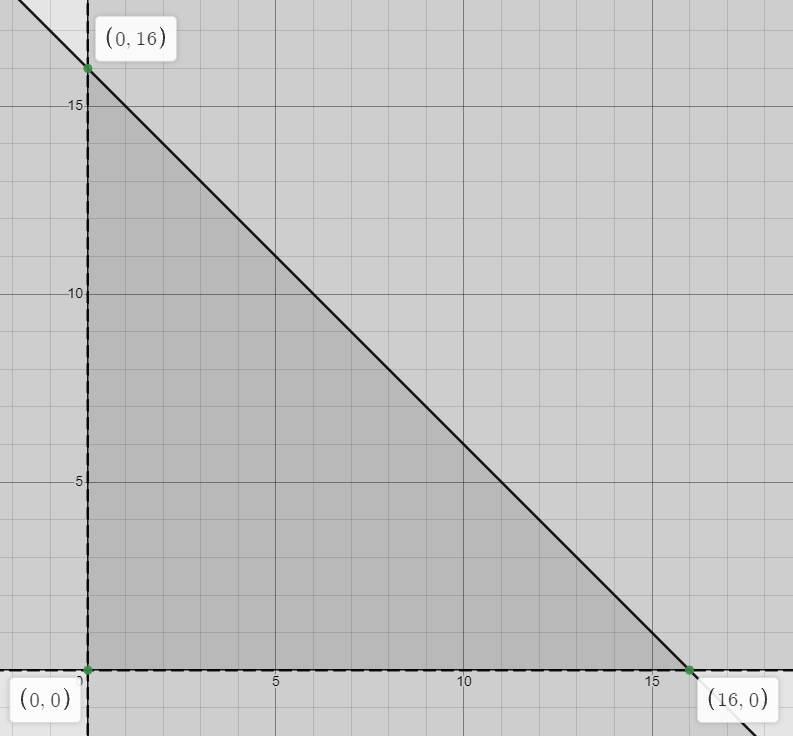
\includegraphics[scale=0.6]{evt_in_3d_graph.png}
\end{center}

Finally, we can compare the found points' satisfaction outputs...
\begin{align*}
	S(4, 4) &= 8\\
	S(0, 4) = \frac{8}{\sqrt[4]{e}} &\approx 6.23041\\
	S(4, 0) = \frac{8}{\sqrt[4]{e}} &\approx 6.23041\\
	S(8, 8) = \frac{8}{\sqrt{e}} &\approx 4.85225\\
	S(0, 0) = \frac{8}{\sqrt{e}} &\approx 4.85225\\
	S(0, 16) = \frac{8}{e^\frac{5}{2}} &\approx 0.65668\\
	S(16, 0) = \frac{8}{e^\frac{5}{2}} &\approx 0.65668\\
\end{align*}

Through all of this work, we found that Joe can still only achieve a maximum satisfaction of $8$ utils!

Do note that, unlike when sweetness was the only option in the $\mathbb{R}^2$ case, Joe does not just want either all sweetness or all umami.
Also note that this is NOT a pattern that holds true for all functions you decide to optimize using the EVT in $\mathbb{R}^3$.

To make this more clear, let's reiterate this multivariable problem-solving concept with another problem.. in the next chapter!
% *: 
\setcounter{chapter}{4}
\chapter{Metonymization, Part 1}
Now, let's try a general example that requires the application of the Extreme Value Theorem in $\mathbb{R}^3$.
\begin{eg}
	Find the absolute minimum and absolute maximum of
	\begin{center}
		$f(x, y) = x^2 - y^2 + xy - 5x$
	\end{center}
	on the region bounded by $y = 5 - x^2$ and the $x$-axis.
\end{eg}

Like when we had to find Joe's maximum satisfaction, we can apply the same techniques!

First, we must find the critical points for $f$, so we set its partial derivatives equal to zero:
\begin{align*}
	f_x(x,y)=2x+y-5&=0\\
	f_y(x,y)=-2y+x&=0
\end{align*}
Then, we solve the system of two equations for two unknowns.

Here, we'll use elimination:
\begin{align*}
	4x+2y&=10\\
	-2y+x&=0\\
	\implies 5x&=10\\
	x&=2
\end{align*}
Doing a bit of algebra yields us with the following:
\begin{align*}
	y=1
\end{align*}
So, we end up with the critical point $(2, 1)$.

Now, we have to find the absolute extrema candidates on the bounds (which we'll infer from the problem statement)!
\begin{enumerate}
	\item $y\leq 5-x^2$
	\item $y\geq 0$
\end{enumerate}

For $1$:
\begin{align*}
	f(x, 5-x^2) &= x^2-(5-x^2)^2+x(5-x^2)-5x\\
	&= -x^4-x^3+11x^2-25
\end{align*}
Find the critical values for $1$:
\begin{align*}
	\frac{\mathrm{d}}{\mathrm{d}x}[f(x, 5-x^2)] = -4x^3-3x^2+22x&=0\\
	\implies x&\in \left\{-\frac{11}{4}, 0, 2\right\}
\end{align*}
And their implied points:
\begin{align*}
	\implies \left\{\left(-\frac{11}{4}, -\frac{41}{16}\right), (0, 5), (2, 1)\right\}
\end{align*}
Note that we can omit $\left(-\frac{11}{4}, -\frac{41}{16}\right)$ because it provides a $y$-value that does not follow relation \#$2$.
We can also ignore the repeated $(2, 1)$ because it already appeared when we used partial derivatives to find the critial point of $f$.

Now for $2$:
\begin{align*}
	f(x, 0) &= x^2-5x\\
\end{align*}
Find its critical values:
\begin{align*}
	\frac{\mathrm{d}}{\mathrm{d}x}[f(x, 0)] = 2x-5&=0\\
	\implies x&=\frac{5}{2}
\end{align*}
And its implied point:
\begin{align*}
	\implies \left(\frac{5}{2}, 0\right)
\end{align*}
Then, find the corner points:
\begin{align*}
	0 = 5-x^2\implies x\in\{-\sqrt{5}, \sqrt{5}\}
	\implies \{(-\sqrt{5}, 0), (\sqrt{5}, 0)\}
\end{align*}
And, finally, we must compare the $f$ values for all found points:
\begin{align*}
	f(2, 1) &= -5\\
	f(0, 5) &= -25\\
	f\left(\frac{5}{2}, 0\right) = -\frac{25}{4} &\approx -6.25\\
	f(-\sqrt{5}, 0) = 5+5\sqrt{5} &\approx 16.18034\\
	f(\sqrt{5}, 0) = 5-5\sqrt{5} &\approx -6.18034
\end{align*}
The amount of work that went into this problem is absurd, but that's fine. In the end, we find that the absolute minimum of $f$ is $-25$ and the absolute maximum is $5+5\sqrt{5}$, or $16.18034$.

This method of finding absolute extrema, given the conditions for EVT in $\mathbb{R}^3$ are held, can be used to:
\begin{itemize}
	\item Optimize stress and strain in $3$D engineering models,
	\item minimize drag and minimize lift in aerodynamic designs,
	\item and analyze historical data patterns regarding natural resource extraction and help companies locate locations with optimal resource quantities. 
\end{itemize}
Moreover, there are many more applications for EVT in $3$D, so long as the $2$D constrained regions of optimization are closed and bounded.

Now wait a second.. what would happen if the $2$D region describing the input of the $3$D function.. is not bounded?
Obviously, we can't apply the Extreme Value Theorem in $\mathbb{R}^3$ in this case.. unless you know how to test all possible points on an unbounded region!
Which, unfortunately, you can't.

Instead, read on...